\documentclass[a4paper,11pt,fleqn, titlepage]{article}

\usepackage[utf8]{inputenc}
\usepackage[swedish]{babel}
\usepackage[lighttt]{lmodern}
\usepackage{parskip}
\usepackage{amsmath}
\usepackage{amssymb}
\usepackage{amsthm}
\usepackage{listings}
\usepackage{graphicx}
\usepackage{biblatex}
\usepackage{csquotes}


\addbibresource{referenser.bib}

\author{Andreas Hagesjö \and Daniel Pettersson \and
Magnus Hagmar \and Niclas Ogeryd \and Robert Nyquist}

\title{Fossilfri bilflotta \\ Kurs ENM155}


\begin{document}
\maketitle

\section{Introduktion}
I denna rapport undersöks möjligheterna för att göra Sveriges bilflotta
fossiloberoende till år 2030. Just nu kommer den största delen av energin
som används i transportsektorn från just fossila bränslen. Detta betyder
såklart att väldigt mycket utsläpp orsakas av alla bilar, utöver den stora
energiförlusten på grund av den låga verkningsgraden för
förbränningsmotorer. Genom att bryta beroendet utav fossila bränslen
förbättras miljön alltså både genom minskade utsläpp och energiförbrukning.

Denna frågeställning är intressant att studera eftersom regeringen har satt
just detta målet för Sverige. Utöver detta så är det både ett aktuellt ämne
i samhället samt att det enligt flera utförda studier går att uppfylla
målsättningen. Denna rapport innehåller en modell som visar vilka energier
som kan användas för att nå detta mål samt olika scenarier för hur målet
kan uppnås. För att det skall vara möjligt så krävs det vissa
ansträngningar och tekniska utvecklingar.

Vad fossiloberoende betyder kan vara en tolkningsfråga, men i denna rapport
används det med betydelsen att det är \emph{möjligt} för bilflottan att
köras på fossilfria bränslen, men att det inte måste vara så. Att ha tillgång
till fossila bränslen och möjlighet att använda det kan vara viktigt för
att upprätthålla bränslesäkerhet ifall det blir en temporär brist på
några av alternativen.

\subsection{El}

För personbilar så kommer eldrift att ersätta stor del av bensin- och
dieseldrift. Då elbilar är effektivare än bilar med förbränningsmotorer så
kommer bytet till elbilar medföra att mängden energi som behöves för att
driva bilflottan att minska \cite[s.~25]{elforsk}. Då stor del utav
elbilarna som säljs idag är laddhybrider, Mitsubishi Outlander står ensam
för nästan 30 procent av det laddbara beståndet i Sverige, så kommer den
typen av bilar fortfarande rulla 2030 och därmed fortfarande använda
fossilt bränsle \cite{laddbarafordon}. I nuläget så är det endast
7800 av de cirka 4.5 miljoner bilarna i sverige som kan drivas på
el \cite{fordonsstatistik}.  Det kommer att diskuteras huruvida 
utvecklingen kan ske till 2030 för att se till att eldrivna bilar kommer
att bli en mer betydande del av fordonsflottan gentemot hur det ser ut
idag, och att efterfrågan för elbilarna kommer att öka drastiskt.
Regeringen har i nuläget infört styrmedel för att gynna elbilar
(och de absolut bästa gasbilarna), med en supermiljöbilspremie, som innebär
att om en bils maximala koldioxidsläpp per kilometer är 50 gram, så kan denna
premie tilldelas \cite{ekonomiskastyrmedel}.
En fråga man kan ställa sig är huruvida det kommer gå att producera den
extra mängden el som behöves för att utöka beståndet med elbilar. Som det
ser ut nu så skulle bilflottan behöva runt 53 TWh/år år 2030 utan några
åtgärder \cite[s.~24]{elforsk}, men med
den effektiviseringen som kommer med elmotorer, mellan 2,5 och 3 gånger så
effektiv \cite[s.~29]{elforsk}, så kommer den
mängden energi att minska så pass mycket att det inte blir nödvändigt med
så stor ökning utav elproduktionen.

\subsection{Biobränsle}
Tunga fordon så som lastbilar och maskiner kommer antagligen inte kunna
köras med eldrivna motorer inom de nästkommande åren, detta på grund av att
man idag inte kan lagra den mängden energi som behövs för att driva ett
stort och tungt fordon. Och eftersom de flesta tunga fordon idag körs på
diesel, kan ett bränslebyte till biodiesel gå relativt smärtfritt.

Samma sak är det med bensin och dieselbilar som säljs idag, eftersom
medelåldern på en personbil i Sverige är 9 år \cite[s.~17]{elforsk} så
betyder det att det kommer köras bilar år 2030 som är sålda idag,
och då måste vi ha ett sätt att med så låg kostnad som möjligt, konvertera
dessa till fossilfria alternativ. Där ligger biobränslen närmast, en bil
som idag körs på diesel, kan som tidigare sagt, relativt smärtfritt köras
på biodiesel istället \cite{statoil}. Lite
svårare bil det däremot med en bensindriven bil. Där kan man bli tvungen
att göra lite större ändringar i motorn, vilket självklart resulterar i en
högre kostnad för konverteringen, men det är mycket möjligt att göra en sån
konvertering. Detta betyder att bilar som säljs idag och några år framåt,
som är avsedda att köras fossila bränslen som bensin och diesel, kan
konverteras och då framföras oberoende av fossila bränslen.

För att främja biobränslet i Sverige har man i nuläget infört ekonomiska styrmedel 
genom att låta allt biobränsle genom att låta dess skatt vara
avdragsgill \cite{ekonomiskastyrmedel}.

Man får dock vara försiktig med just biobränslen, det finns inte
biobränslen i överflöd, och skulle andra länder få en ökad efterfrågan på
biobränslen kan det få priset att rusa i taket. Detta kan medföra stora
negativa effekter så som \emph{land-grabbing} \cite{bioenergi}, ökade matpriser i
fattigare länder etc. vilket man då kan reglera genom att man har kvar
möjligheten att tillfälligt köra på fossila bränslen, för att minska
Sveriges efterfrågan på biobränslen dels ur bränslesäkerhet men även
miljömässigt och kanske även ur ett etiskt perspektiv.

\subsection{Vätgas}
Bilar som drivs på vätgas ligger för tillfället bakom både elbilar och
bilar som drivs på biobränsle och därför räknar vi med att år 2030 så
består inte stora delar utav bilflottan av bilar som drivs av vätgas.
Bilarna produceras fortfarande i små mängder och i sverige finns endast en
laddningsstation för tillfället \cite{macken}.
Bilarna är dessutom fortfarande för dyra för att få ett stort genomslag än så länge. Bilar som drivs på vätgas har har stor potential i framtiden men 2030 så kommer de inte finnas i lika stor mäng som elbilar och biobränsle bilar.

\subsection{Kärnkraft}
Regerigen har upphävt förbudet mot ny kärnkraft i Sverige. Detta har lett till intresse till ersätta gamla reaktorer med nya, bland annat i Oskarshamn, som kan producera mer el.
Dessutom så kan man räkna med att samtliga aktiva reaktorer i Sverige
kommer att producera en större mängd el om 15 år än vad de gör nu
\cite[s.~80]{karnkraft}. Därför räknar vi med att kärnkraften år 2030 har möjlighet att täcka upp för det ökade behovet utav elproduktion som en ökad mängd elbilar medför.

\section{Metod}
Vi har utgått från den angivna modellen i tidigare uppgift. Med den som
ursprungsläge samt information från flera rapporter och prognoser i ämnet
har vi kunnat få fram en hypotes till hur energisystemet kan komma att se
ut 2030. Vi har sen matat vår algoritm med hypotesen, den har sen räknat ut
resultatet och visar det i den form som vi behöver.

\begin{figure}[h!]
	\centering
	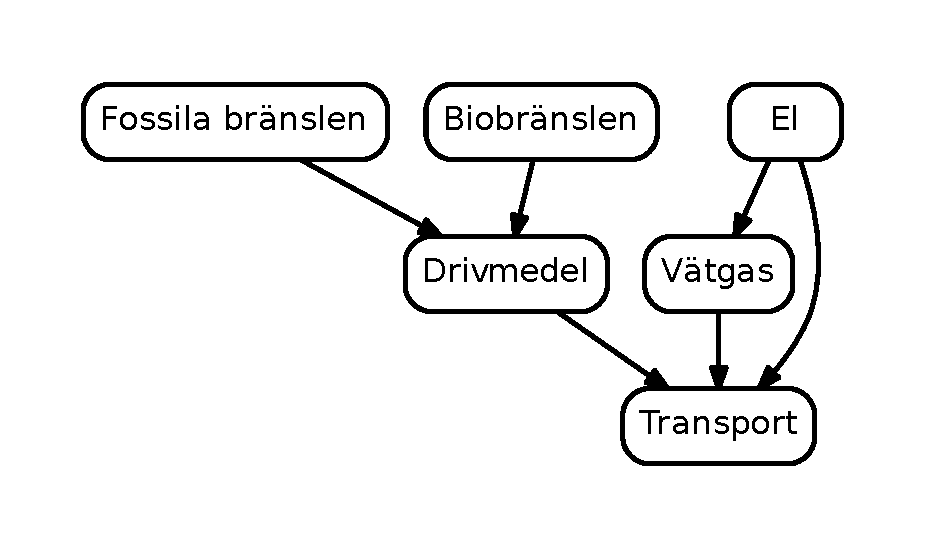
\includegraphics[scale=0.70]{diagram.pdf}
	\label{modell}
	\caption{Förenklad modell av transportsektion.}
\end{figure}

Den nuvarande modellen över transportsektorn ser förenklad ut som i figur
\ref{modell}. På pilarna mellan lådorna ska det såklart vara
transmissionsförluster och verkningsgrader, men eftersom dessa varierar i
de olika scenarierna har vi valt att inte skriva ut dessa.

Fördelen med vårt tillvägagångssätt är att vi kan vara säkra på att vårt
resultat är korrekt beräknat då vi har matematiken att falla tillbaka på.
Så resultatet från vår algoritm är korrekt, en nackdel är dock att vi inte
kan vara säkra på att vår indata till algoritmen är korrekt. Det är
omöjligt för oss att säga hur verkligheten kommer att se ut 2030. Hypotesen
vi har är så realistisk som vi kunde få den till med hjälp av den datan som
vi kommit över. Vi har inte räknat med några stora oförutsedda scenarion,
utan mer eller mindre räknat med att övriga områden ska fortsätta utvecklas
som vanligt.


\section{Resultat}

\subsection{Scenario 1 - Biobränslen och elbilar}

För att ersätta fossila bränslen så är som bekant de två huvudalternativen
biobränslen eller elbilar. I detta scenario så utvecklas både användningen
av biobränslen, samtidigt som en del av bilflottan byts ut mot el- eller
hybridbilar.

Enligt Regeringens utredning 2013 så kan energianvändningen hos
förbränningsmotorer för personbilar väntas minska med ca 28 procent till år
2030 \cite{fossilfrihet}. Denna utveckling gör att verkningsgraden utav
drivmedel ökar med åtta procentenheter från 20 till 28\%.  Totalt sett så
kan energianvändningen för personbilar väntas minska med 43-50\% om elbilar
och laddhybrider vid eldrift står för drygt 40 procent av körsträckan
\cite{fossilfrihet}.  Energianvändningen minskar dock inte lika mycket som
den eftersom verkningsgraden för att framställa drivmedel utav biomaterial
är 45\% lägre än för fossila bränslen.

Bilar som drivs helt eller delbart med el förväntas göra så att el står för
någonstans mellan 3 och 14 procent av den totala energianvändningen hos
vägtrafiken.

Energianvändningen för tunga fordon, sjöfart, bantrafik samt flyg förväntas
minska något också, då de förväntas ha en effektivisering på 10-14 procent.
Just nu står vägtrafiken för 94\% av hela sektorns förbrukade energi, och
om de olika trafikslagen upptar lika stor andel av transportsektorns
förbrukning år 2030 som nu så kommer energianvändningen se ut som i tabell
\ref{tab:scen1energi}.

\begin{figure}[h!]
	\begin{center}
	\begin{tabular}{ | l | l | l | }
	\hline
						& Nu		& 2030 \\ \hline
	Fossil energi				& 94 TWh	& 22,2 TWh \\ \hline
	Biobränsle				& 11 TWh	& 60 TWh \\ \hline % 91% av energianvändningen
	El					& (Nästan) 0 TWh &  2,2 TWh \\ \hline % ~6% av bilenergianvändningen
	Total energianvändning		& 105 TWh	& 86 TWh \\ \hline
	Energianvändning av personbilar	& 50 TWh	& 35 TWh \\ \hline
	\end{tabular}
	\caption{yoloswag}
	\label{tab:scen1energi}
\end{center}
\end{figure}



Det största användingsområdet för biomassa är i nuläget uppvärmning, om man istället använde
I Sverige finns det stora mängder mark som kan användas för att odla biomassa. En kraftigt ökad produktion, i samband med ett utbyte av fossila bränslen och biodrivmedel för uppvärmning möjliggör en ökning av bio-fordon. Existerande fordon kan även utrustas med teknologi som gör att de kan drivas med biobränslen.

En stor del av uppvärmningen sker idag genom biovärme, om mängden biomassa som används för uppvärmning istället används inom produktion av biodrivmedel. Uppvärmingen skall istället ske med hjälp av el, detta innebär att elproduktionen måste ökas markant. För att tillgodose dessa energibehov ska kärnkraften utökas. Sverige har stora mängder uran som skulle användas som bränsle, dessutom ger kärnkraft stora mängder energi för en relativt liten mängd bränsle. På grund av de stora mängderna el som produceras så kommer det även finnas tillräckligt mycket för att ladda en ökad mängd elbilar.


\section{Diskussion}

\subsection{Scenario 1}
Scenario 1 är möjligt att genomföra på flera olika sätt och här kommer det diskuteras två olika lösningar. 
Det finns vissa gemensamma problem och åtagande för båda lösningarna.

Ökad användning utav biobränsle är ett måste. Detta behöver man vara väldigt försiktig med i början, då ökad produktion måste göras i kontrollerade mängder så det inte leder till höjda markpriser vilket kan bidra till ökad pris på mat och land-grabbing.
Enligt regeringens rapport så kommer Sverige att kunna producera 50-60 TWh mer biomassa per år, vilket motsvarar 25-30 TWh mer biodrivmedel jämfört med dagens mängd. Detta kommer förmodligen inte att vara tillräckligt för att täcka det behovet som en stor utökning utav bilar som drivs på biodrivmedel orsakar, alltså kan Sverige komma att behöva importera biomassa från anda länder.

Mängden el som kommer användas samt behöva produceras ändras med dessa genomföranden och detta är möjligt att göra på olika sätt, vilket diskuteras i de olika alternativen.

Det är inte bara mängden energi och fördelningen som måste lösas utan man måste även övertyga sveriges bilförare om att bilar som drivs av biodrivmedel och el är en bra och effektiv lösning.
Det får inte finnas en ekonomisk förlust för personer som väljer dessa typer av bilar ifall man vill öka antalet användare utav denna typ av bil. Detta problem kan staten hjälpa till med genom att exempelvis fortsätta med skatteavdraget och avdrag på trängselskatt.

Det behöves även styrmedel för att underlätta användningen utav miljöbilar. Bensinstationer behöver erbjuda möjligheten att tanka med biobränsle och att ladda sin elbil. Regler för laddningsstationer när nya parkeringplatser byggs skulle göra användningen utav elmotorer smidigare och problemet med räckvidden skulle minska.

En viktig del kan bli att göra kollektivtraffiken mer konkurrenskraftig. Att planering utav infrastrukturer gynnar användning utav kollektivtrafik så att bilar används i mindre utsträckning och därmed minskar energin som behöves för att driva bilflottan och hela transportflottan totalt.

\subsubsection{Alternativ 1}
Här görs ett utbyte mellan biobränsle som används till uppvärmning och fossila bränsle som används till drivmedel för personbilar. Detta kommer inte lösa några problem då fossila bränslen fortfarande kommer användas inom ett annat område. Samtidigt kommer det skapa större energiförluster då biobränsle har högre verkningsgrad i omvandling till värme jämfört med drivmedel. Fossila bränsle har söttre verkningsgrad i omvandling till drivmedel jämfört med värme. Dessa förluster kan täckas med el. Ökningen utav elbilar gör att biobränslet inte behöver ge samma mängd energi som fossila bränslen gav. Fossila bränslen och biobränslen har samma verkningsgrad när de används till uppvärmning så där kommer det inte vara några energiförluster som behöver täckas upp.

Att de fossila bränslet flyttas från ett område till ett annat kan i detta fall hjälpa till med att minska den fossila användningen totalt. Att plocka bort den fossila användningen i trafik är en viktigt och komplex del i att minska vårt beroende av fossila bränslen. Så att till en början använda mer fossila bränslen är inget stort problem då det med tiden kommer att fasas ut genom att exempelvis använda förnyelsebar el som uppvärmning. Detta kommer fördröja avvecklingen, men hjälpa till med att skapa en fossilfri bilflotta.

\subsubsection{Alternativ 2}

Idag används mycket biobränsle till uppvärmning. Om man istället börjar använda denna mängd till att tillverka drivmedel så kan det ersätta stora delar utav det fossila bränslet. Det kommer då behövas energier från andra källor för att ersätta biobränslet i andra sektorer. Detta skulle kunna ersättas med el. För att detta skall vara möjligt behöver sveriges elproduktion öka till 2030. Sveriges riksdagen har en planeringsram till år 2020 om att öka elproduktionen från 10 TWh till 30 TWh, en siffra som förmodligen kommer att vara ännu högre år 2030. Dessutom så räknas sveriges reakatorer producera mer el 2030 än va de gör idag om inga reaktorer stängs ner.


\subsection{Scenario 2}
I litteraturen så har vätgasbilar väldigt liten inverkan på bilflottan 2030 (KOLLA DETTA), dessutom så har finns det flera större rapporter där alla pekar på att antalet vätgasbilar kommer vara marginell.
Då utvecklingen utav vätgasbilar fortfarande är i ett stadie där det experimenteras mycket och modellerna endast finns i små mängder så har de ett väldigt högt inköpspris. För att vätgasbilar skall finnas i en större utbredning år 2030 så måste bilföretag välja att börja producera i större skalor så att priserna går ner.

Statliga medel som tvingar fram tankstationer är också ett måste då det för tillfället endast finns en tankstation i Malmö och två planerade, en vadera i Stockholm och Göteborg.
Ekonomiska medel från staten skulle göra att försäljningen kan öka tidigare då försäljningspriset kan vara högra utan att direkt påverka privatpersoners ekonomi.
Tyskland, Japan och Karlifonien är de platser där uppbyggnaden utav vätgasstationer har kommit längst. Där har myndigheter sammarbetat med företag för att dela på kostnader och risker som det innebär. Sådana sammarbeten skulle även behövas i Sverige om man snabbt vill bygga upp en infrastruktur som stödjer vätgasbilar.

Något som talar för att utvecklingen för vätgasbilar skall gå framåt i snabbt takt är att det forskars på att använda vätgas som lagring för energi från exempelvis vindkraftverk. Detta skulle göra vindkraft mindre beroende av andra energikällor när det inte blåser. Utvecklingen av att binda energi i vätgas har alltså fördelar i andra områden än transport vilket gör att forskning inom området är lönsamt för flera. Det finns även industrier som har vätgas som spillvara som man kan ta vara å för att få vätgas direkt utan några energiförluster vid tillverkningen.


\printbibliography
\end{document}

